\documentclass[11pt]{article}
\usepackage[margin=1in]{geometry}
\usepackage{amsmath,amssymb}
\usepackage{booktabs}
\usepackage{graphicx}
\usepackage[numbers]{natbib}
\usepackage{hyperref}

\graphicspath{%
  {./}%
  {../results/neural_sde_comparison_outputs/}%
  {../results/all_model_comparison_outputs/}%
  {../results/logistic_pinn_outputs/}%
  {../results/neural_ode_outputs/}%
}

\newcommand{\comparisonfigurewidth}{0.96\textwidth}
\newcommand{\diagnosticfigurewidth}{\textwidth}

\title{Comparison of Classical, Neural ODE/SDE, and Logistic PINN Fits for Water Kefir Data}
\author{Saul Diaz-Infante Velasco}
\date{}

\begin{document}
\maketitle

\begin{abstract}
    This report compares five dynamical descriptions of water kefir
    fermentation data: a classical logistic ordinary differential equation, a
    deterministic Neural ODE, a Neural SDE, a deterministic logistic PINN, and a
    stochastic logistic PINN/SDE. The data consist of three trials measured at
    15 time points, giving 45 scalar observations. The Neural ODE and the two
    logistic PINNs are treated as population models: the three trials are
    interpreted as repeated realizations of the same experiment, so one fitted
    curve is compared with all trial observations. The stochastic logistic PINN
    additionally identifies a multiplicative diffusion parameter and generates
    Monte Carlo predictive intervals. The reported residual criteria are
    in-sample diagnostics; out-of-sample MSE should be computed with a
    time-respecting train/test split.
\end{abstract}

\section{Data and preprocessing}

        Let $y_i^{[j]}$ denote the response observed at time $t_i$ in trial $j$,
    with $i=0,\ldots,T-1$ and $j=1,\ldots,J$. In this experiment $T=15$ and
    $J=3$. The time points run from $0$ to $168$ in the original time units.
    The observed index set is
    $$
    \Omega = \{(i,j): y_i^{[j]}\ \hbox{is observed}\},
    \qquad n = |\Omega| = 45.
    $$

        The Neural ODE and Neural SDE were trained on normalized time and
    normalized response:
    $$
        \tau_i = \frac{t_i-t_{\min}}{t_{\max}-t_{\min}},
        \qquad
        z_i^{[j]} = \frac{y_i^{[j]}-\bar y}{s_y},
    $$
    where
    $$
        \bar y = \frac{1}{n}\sum_{(i,j)\in\Omega} y_i^{[j]},
        \qquad
        s_y =
            \left[
                \frac{1}{n}\sum_{(i,j)\in\Omega}(y_i^{[j]}-\bar y)^2
            \right]^{1/2}.
    $$
    Thus $\tau_i\in[0,1]$. The logistic PINN models also use normalized time,
    but their neural trajectories are expressed directly on the original
    response scale. Their data and physics losses are divided by $s_y^2$ so
    that residual terms are dimensionless and numerically comparable. All model
    diagnostics were computed on the original response scale; for the Neural
    ODE and Neural SDE this required transforming fitted normalized values back
    to the scale of $y_i^{[j]}$.

\section{Models}

    \subsection{Classical logistic ODE}
            The classical baseline is the Verhulst logistic growth model
        \citep{verhulst1838notice}, fitted here as a shared-parameter nonlinear
        regression model. Unlike the neural models, it is fitted directly to the
        original response values $y_i^{[j]}$. The only normalization used by
        this baseline is the normalized time variable $\tau_i\in[0,1]$. Each
        trial has its own observed initial condition, fixed at the first
        measured value, but all trials share the same growth rate and carrying
        capacity:
        $$
            \frac{d y^{[j]}}{d\tau}
            =
            r y^{[j]}\left(1-\frac{y^{[j]}}{K}\right),
            \qquad
            y^{[j]}(0)=y_0^{[j]}=y^{[j]}(t_0).
        $$
        The exact solution used in the fit is
        $$
            y^{[j]}(\tau)
            =
                \dfrac{K}{
                    1 +
                    \left(
                        \dfrac{K - y_0^{[j]}}{ y_0^{[j]} }
                    \right)
                    \exp(-r\tau)
                }.
        $$
        The unknown parameters of the classical fit are only $r$ and $K$; the
        initial values $y_0^{[j]}$ are taken from the data and are not
        optimized. The fit also requires positive observations, because the
        closed-form logistic curve and the ratio $(K-y_0^{[j]})/y_0^{[j]}$ are
        only meaningful for positive initial values.
        Missing observations, if present, are excluded through the observed
        index set $\Omega$.

            The fitted parameters must satisfy $r>0$ and $K>\max_j y_0^{[j]}$.
        Instead of optimizing constrained parameters directly, the
        implementation optimizes two unconstrained real variables
        $a, b \in\mathbb R$ and maps them to valid physical parameters with a
        $\operatorname{softplus}$ transformation:
        $$
            r = \operatorname{softplus}(a)+10^{-6},
                \qquad
                K = K_{\min} +
                \operatorname{softplus}(b)+10^{-6},
        $$
        where $K_{\min}=\max_j y_0^{[j]}+10^{-3}$ and
        $$
            \operatorname{softplus}(x)=\log(1+\exp(x)).
        $$
        The $\operatorname{softplus}$ function is a smooth differentiable
        approximation to the positive part function. It maps every real number
        to a positive value, behaves approximately like $\exp(x)$ for large
        negative $x$, and behaves approximately like $x$ for large positive
        $x$. This is useful for gradient-based fitting:
        Adam can update the unconstrained variables $a$ and $b$ freely, while
        the reported parameters $r$ and $K$ remain positive and the carrying
        capacity stays above every initial condition. The small constants
        $10^{-6}$ and $10^{-3}$ are numerical safeguards that avoid zero growth
        and avoid a carrying capacity equal to an initial value.

The raw parameters are initialized by applying the inverse softplus map. In the
implementation, this gives an initial growth rate near $3.0$ on the normalized
time scale, and an initial carrying capacity slightly above the largest
observed response. At each training epoch the code applies the softplus
transformation and evaluates the exact logistic solution for all trials and all
observation times.

The fitting criterion is the masked original-scale mean squared error
$$
  \mathcal L_{\mathrm{logistic}}(r,K)
  =
  \frac{1}{n}
  \sum_{(i,j)\in\Omega}
  \left(y_i^{[j]}-\widehat y^{[j]}(\tau_i)\right)^2.
$$
This can also be interpreted as a maximum-likelihood fit after adding a
Gaussian observation-error model on the original response scale:
$$
  y_i^{[j]}
  =
  \widehat y^{[j]}(\tau_i;r,K)+\varepsilon_i^{[j]},
  \qquad
  \varepsilon_i^{[j]}\stackrel{\mathrm{ind}}{\sim}
  \mathcal N(0,\sigma^2).
$$
For fixed $\sigma^2$, maximizing this Gaussian likelihood over $r$ and $K$ is
equivalent to minimizing the sum of squared residuals. If $\sigma^2$ is also
unknown, profiling it out gives
$$
  \widehat\sigma^2(r,K)
  =
  \frac{1}{n}
  \sum_{(i,j)\in\Omega}
  \left(y_i^{[j]}-\widehat y^{[j]}(\tau_i;r,K)\right)^2,
$$
and the maximizing values of $r$ and $K$ are again the nonlinear least-squares
solution. Therefore the implemented classical fit is a profiled Gaussian
maximum-likelihood estimate under an independent additive measurement-error
assumption. It is not a transition likelihood for a stochastic logistic process.

The code backpropagates through the closed-form expression above and applies an
Adam update \citep{kingma2015adam} to $a$ and $b$. No numerical ODE solver is
used for this classical baseline. This model was trained for 3000 Adam epochs
with learning rate $5\times10^{-2}$.

The inverse-problem procedure for this classical logistic model is therefore:
\begin{enumerate}
  \item Read the observed trial matrix and keep only entries in $\Omega$.
  \item Fix the initial condition of each trial at its observed first value
        $y_0^{[j]}$; these initial values are not optimized.
  \item Choose unconstrained optimization variables $a$ and $b$, and transform
        them into admissible physical parameters $r(a)>0$ and $K(b)>K_{\min}$
        with the softplus maps above.
  \item For the current values of $a$ and $b$, compute the exact logistic curve
        $\widehat y^{[j]}(\tau_i;r,K)$ for every trial and observation time.
  \item Evaluate the masked residual objective
        $\mathcal L_{\mathrm{logistic}}(r,K)$, using only observed entries.
  \item Use automatic differentiation through the closed-form solution to
        compute $\partial \mathcal L_{\mathrm{logistic}}/\partial a$ and
        $\partial \mathcal L_{\mathrm{logistic}}/\partial b$.
  \item Apply an Adam step to $a$ and $b$, then repeat until the fixed epoch
        budget is reached.
  \item Report $\widehat r=r(\widehat a)$ and
        $\widehat K=K(\widehat b)$, and evaluate fitted curves and residual
        metrics on the original data scale.
\end{enumerate}

In this baseline the inverse problem is low-dimensional: only two unknown
physical parameters are estimated. The use of gradient descent is an
implementation choice; mathematically, the estimator is the nonlinear
least-squares solution for the two-parameter logistic curve under fixed
trial-specific initial conditions.
The fitted values were
$$
  \widehat r = 7.705769,
  \qquad
  \widehat K = 47.860203.
$$
Since $\tau=t/168$ for these data, the growth rate in the original time scale
is approximately $\widehat r/168=0.045868$ per original time unit.

\subsection{Neural ODE}

The deterministic neural model is the non-autonomous Neural ODE
\citep{chen2018neuralode}
$$
  \frac{d z}{d\tau} = f_\theta(\tau,z),
  \qquad
  z(0)=z_0.
$$
The fitted solution is a single population curve, not one curve per trial. The
three trials are treated as replicate observations of the same underlying
trajectory. On the original response scale the initial condition is
$$
  y_0 = y(t_0)
  =
  \frac{1}{J}\sum_{j=1}^J y_0^{[j]},
$$
the mean of the first observed values across trials. The corresponding
normalized initial condition is
$$
  z_0 = \frac{y_0-\bar y}{s_y}.
$$
After solving the normalized ODE, the fitted value on the original scale is
$$
  \widehat y_i
  =
  \widehat y(t_i)
  =
  \bar y+s_y\widehat z(\tau_i;\theta).
$$
The same value $\widehat y_i$ is compared with every trial observation
$y_i^{[j]}$ at time $t_i$.

The right-hand side $f_\theta$ is a fully connected neural network with input
$(\tau,z)\in\mathbb R^2$, two hidden layers, 32 hidden units per layer, and
hyperbolic tangent activation:
$$
  h_1 = \tanh(W_1 x+b_1),\qquad
  h_{\ell}=\tanh(W_{\ell}h_{\ell-1}+b_{\ell}),\qquad
  f_\theta(x)=W_o h_2+b_o,
$$
where $x=(\tau,z)^T$. The network has 1185 trainable weights and biases.
This count comes from the three affine layers:
$$
\begin{aligned}
  \hbox{input to hidden 1:}&\quad 2\cdot 32+32=96,\\
  \hbox{hidden 1 to hidden 2:}&\quad 32\cdot 32+32=1056,\\
  \hbox{hidden 2 to output:}&\quad 32\cdot 1+1=33.
\end{aligned}
$$
Thus $96+1056+33=1185$. The architecture was chosen as a compact smooth
function approximator for a scalar time-dependent vector field. The input has
only two coordinates, time and state, and the data set has only 45 scalar
observations, so a very large network would make the comparison dominated by
overparameterization. Two hidden layers with 32 units give substantially more
flexibility than the two-parameter logistic curve while remaining small enough
to train stably with weight decay. The $\tanh$ nonlinearity gives a smooth
right-hand side, which is useful for ODE/SDE integration, and sigmoidal neural
networks are classical universal approximators \citep{cybenko1989approximation}.
The same architecture is used for the Neural ODE and for each Neural SDE
coefficient so that differences between the deterministic and stochastic neural
models are not caused by different network sizes.

The ODE was solved at the observed normalized times using RK4 with step size
$0.01$. The empirical loss was
$$
  \mathcal L_{\mathrm{ODE}}(\theta)
  =
  \frac{1}{n}
  \sum_{(i,j)\in\Omega}
  \left(z_i^{[j]}-\widehat z_i(\theta)\right)^2.
$$
Equivalently, in original response units this loss fits one curve
$\widehat y_i$ to all three replicate measurements at the same time. The
minimizer is therefore encouraged to pass through the center of the replicate
cloud, while the ODE structure enforces a smooth dynamical trajectory.
Training used Adam for 1000 epochs with learning rate $10^{-2}$ and weight
decay $10^{-4}$ \citep{kingma2015adam}.

\subsection{Neural SDE}

The stochastic neural model is an Ito diffusion with neural drift and diffusion
coefficients, following the Neural SDE modeling idea
\citep{tzen2019neuralsde,kidger2021neuralsdegan}:
$$
  dZ_\tau
  =
  \mu_\theta(\tau,Z_\tau)\,d\tau
  +
  \sigma_\phi(\tau,Z_\tau)\,dW_\tau.
$$
Both the drift $\mu_\theta$ and the raw diffusion network use the same
architecture as the Neural ODE: two hidden layers, 32 units per hidden layer,
and $\tanh$ activation. The diffusion is constrained to be positive by
$$
  \sigma_\phi(\tau,z)
  =
  \operatorname{softplus}(g_\phi(\tau,z))+\sigma_{\min},
  \qquad
  \sigma_{\min}=10^{-3}.
$$
The total trainable parameter count is 2370, one copy of the 1185-parameter
network for the drift and one for the diffusion.

The SDE was trained with an Euler-Maruyama Gaussian transition likelihood
\citep{kloeden1992numerical}. For successive observations separated by
$\Delta\tau_i=\tau_{i+1}-\tau_i$, the approximation is
$$
  Z_{i+1}^{[j]}\mid Z_i^{[j]}
  \sim
  \mathcal N\left(
    Z_i^{[j]}+\mu_\theta(\tau_i,Z_i^{[j]})\Delta\tau_i,\,
    \sigma_\phi(\tau_i,Z_i^{[j]})^2\Delta\tau_i
  \right).
$$
With the variance floor used in the implementation, define
$$
  m_i^{[j]}=z_i^{[j]}+\mu_\theta(\tau_i,z_i^{[j]})\Delta\tau_i,
  \qquad
  v_i^{[j]}=\sigma_\phi(\tau_i,z_i^{[j]})^2\Delta\tau_i+10^{-6}.
$$
The minimized negative log-likelihood is
$$
  \mathcal L_{\mathrm{SDE}}(\theta,\phi)
  =
  \frac{1}{|\Omega_{\mathrm{tr}}|}
  \sum_{(i,j)\in\Omega_{\mathrm{tr}}}
  \frac{1}{2}
  \left[
    \log(2\pi v_i^{[j]})
    +
    \frac{(z_{i+1}^{[j]}-m_i^{[j]})^2}{v_i^{[j]}}
  \right],
$$
where $\Omega_{\mathrm{tr}}$ is the set of adjacent observed transitions.
Training used Adam for 1000 epochs with learning rate $5\times10^{-3}$ and
weight decay $10^{-4}$ \citep{kingma2015adam}. After training, 1000 Monte Carlo
paths were simulated to estimate predictive means and central 90 percent
intervals.

\subsection{Logistic PINN inverse models}

The two new models solve the inverse problem for the logistic growth law with a
physics-informed neural network (PINN) \citep{raissi2019physics}. Unlike the
classical logistic baseline, the PINN does not evaluate the closed-form
logistic solution during training. Instead, it learns a neural trajectory
$u_\eta(\tau)$ and estimates the physical parameters by penalizing violations
of the differential equation.

The unknowns in the deterministic PINN inverse problem are
$$
  \eta,\quad r,\quad K,
$$
where $\eta$ denotes all neural-network weights and biases. The unknowns in the
stochastic PINN inverse problem are
$$
  \eta,\quad r,\quad K,\quad \sigma.
$$
The role of the neural trajectory $u_\eta$ is to provide a differentiable
surrogate for the unobserved continuous-time biomass curve. The physical
parameters are then identified by forcing this differentiable surrogate to
match the measurements and to satisfy the logistic differential equation at
collocation points between measurements. This is the main distinction from the
closed-form classical logistic fit: the PINN estimates a curve and the
parameters jointly.

\subsubsection{Shared PINN trajectory architecture}

Both logistic PINNs use a scalar neural trajectory
$$
  u_\eta:[0,1]\rightarrow \mathbb R_+,
  \qquad
  \widehat y(t)=u_\eta(\tau(t)).
$$
The network input is the normalized time $\tau$. The hidden architecture has
three fully connected hidden layers, 32 units in each hidden layer, and
hyperbolic tangent activation:
$$
  h_1=\tanh(W_1\tau+b_1),\qquad
  h_\ell=\tanh(W_\ell h_{\ell-1}+b_\ell),\quad \ell=2,3,
$$
followed by one scalar output layer. Positivity of the fitted biomass
trajectory is enforced by
$$
  u_\eta(\tau)=\operatorname{softplus}(W_o h_3+b_o)+10^{-6}.
$$
The trajectory network has 2209 trainable weights and biases:
$$
\begin{aligned}
  \hbox{input to hidden 1:}&\quad 1\cdot 32+32=64,\\
  \hbox{hidden 1 to hidden 2:}&\quad 32\cdot 32+32=1056,\\
  \hbox{hidden 2 to hidden 3:}&\quad 32\cdot 32+32=1056,\\
  \hbox{hidden 3 to output:}&\quad 32\cdot 1+1=33.
\end{aligned}
$$
Thus the deterministic logistic PINN has $2209+2=2211$ fitted parameters after
adding the raw variables for $r$ and $K$, while the stochastic logistic PINN
has $2209+3=2212$ fitted parameters after adding the raw variable for
$\sigma$.

The carrying capacity is constrained to remain above all observed responses,
not only above the first row. Define
$$
  K_{\min}=\max_{(i,j)\in\Omega} y_i^{[j]}+10^{-3}.
$$
The deterministic PINN optimizes unconstrained variables $a,b\in\mathbb R$ and
maps them to physical parameters by
$$
  r=\operatorname{softplus}(a)+10^{-8},
  \qquad
  K=K_{\min}+\operatorname{softplus}(b)+10^{-8}.
$$
The stochastic PINN adds a third unconstrained variable $c$ and uses
$$
  \sigma=\operatorname{softplus}(c)+10^{-8}.
$$
Here $r$ is on the original time scale, because the physics residual includes
the time-scale factor $t_{\max}-t_{\min}=168$.

The PINN initialization is chosen to start from a stable positive trajectory.
The final network layer is initialized so that $u_\eta(\tau)$ is approximately
constant at the mean observed initial level,
$$
  \bar y_0=\frac{1}{J}\sum_{j=1}^J y_0^{[j]}.
$$
The initial carrying capacity is set slightly above the largest observed
response, and the initial growth rate is estimated from the first and last
observed means using the analytic logistic relationship. If that estimate is
not admissible, a small positive default value is used. The stochastic fit
starts from a positive multiplicative diffusion value, $\sigma=0.02$, before
gradient-based optimization.

\subsubsection{Deterministic logistic PINN}

The deterministic inverse problem is based on the original-time logistic ODE
$$
  \frac{dX}{dt}=rX\left(1-\frac{X}{K}\right).
$$
Since the PINN is differentiated with respect to normalized time $\tau$, the
residual uses
$$
  \frac{du_\eta}{d\tau}
  =
  (t_{\max}-t_{\min})\,
  r u_\eta(\tau)\left(1-\frac{u_\eta(\tau)}{K}\right).
$$
Let $\{\xi_m\}_{m=1}^M$ be $M=128$ uniformly spaced collocation points in
$[0,1]$. The data, initial-condition, and physics losses are
$$
  \mathcal L_{\mathrm{data}}(\eta)
  =
  \frac{1}{n}
  \sum_{(i,j)\in\Omega}
  \left(
    \frac{u_\eta(\tau_i)-y_i^{[j]}}{s_y}
  \right)^2,
$$
$$
  \mathcal L_{\mathrm{init}}(\eta)
  =
  \frac{1}{J}
  \sum_{j=1}^J
  \left(
    \frac{u_\eta(0)-y_0^{[j]}}{s_y}
  \right)^2,
$$
and
$$
  \mathcal L_{\mathrm{phys}}(\eta,r,K)
  =
  \frac{1}{M}
  \sum_{m=1}^M
  \left[
    \frac{
      \dfrac{du_\eta}{d\tau}(\xi_m)
      -
      (t_{\max}-t_{\min})r u_\eta(\xi_m)
      \left(1-\dfrac{u_\eta(\xi_m)}{K}\right)
    }{s_y}
  \right]^2 .
$$
The deterministic PINN objective is
$$
  \mathcal L_{\mathrm{detPINN}}
  =
  \mathcal L_{\mathrm{data}}
  +
  \lambda_0\mathcal L_{\mathrm{init}}
  +
  \lambda_{\mathrm{phys}}\mathcal L_{\mathrm{phys}},
$$
with $\lambda_0=1$ and $\lambda_{\mathrm{phys}}=1$ in the reported run. This
fit uses one population trajectory against all three replicate trials. It is
therefore more flexible than the classical two-parameter logistic regression,
because the neural trajectory can absorb deviations from the exact analytic
curve, but it is still regularized toward the logistic differential equation.
Training used Adam for 3000 epochs with learning rate $5\times10^{-3}$.

The deterministic PINN inverse problem is solved by the following optimization
loop:
\begin{enumerate}
  \item Build the observation tensor, mask missing entries, compute $s_y$, and
        map observation times to $\tau_i\in[0,1]$.
  \item Create the collocation grid
        $\xi_1,\ldots,\xi_M$ on $[0,1]$. These points are not additional data;
        they are locations where the logistic differential equation is
        enforced.
  \item Initialize the trajectory network $u_\eta$ and raw physical variables
        $a,b$. The reported parameters at every epoch are obtained from
        $r=\operatorname{softplus}(a)+10^{-8}$ and
        $K=K_{\min}+\operatorname{softplus}(b)+10^{-8}$.
  \item Evaluate the population trajectory at the observation times to compute
        $\mathcal L_{\mathrm{data}}$ and $\mathcal L_{\mathrm{init}}$.
  \item Evaluate $u_\eta(\xi_m)$ at the collocation points and use automatic
        differentiation to compute $du_\eta/d\tau$ at those same points.
  \item Form the residual
        $du_\eta/d\tau-(t_{\max}-t_{\min})r u_\eta(1-u_\eta/K)$ and compute
        $\mathcal L_{\mathrm{phys}}$.
  \item Add the weighted terms to obtain
        $\mathcal L_{\mathrm{detPINN}}$, backpropagate through both the
        network and the softplus-transformed parameters, and update
        $(\eta,a,b)$ with Adam.
  \item After training, transform the final raw variables to
        $\widehat r$ and $\widehat K$, and evaluate $u_{\widehat\eta}(\tau)$
        on the observed and dense plotting grids.
\end{enumerate}

The gradients with respect to $r$ and $K$ are not computed by finite
differences. They are obtained by automatic differentiation through the loss
terms. In particular, the physics loss connects $r$ and $K$ directly to the
neural trajectory derivative, so the fitted parameters are those that make the
learned curve both close to the observations and dynamically consistent with
logistic growth.

\subsubsection{Stochastic logistic PINN/SDE}

The stochastic inverse problem augments the same logistic drift with
multiplicative process noise:
$$
  dX_t
  =
  rX_t\left(1-\frac{X_t}{K}\right)\,dt
  +
  \sigma X_t\,dW_t .
$$
The stochastic PINN retains the same neural trajectory, data loss, initial
loss, and physics residual used by the deterministic PINN. The additional
identification of $\sigma$ comes from an Euler-Maruyama transition likelihood
on adjacent observed pairs. For $\Delta t_i=t_{i+1}-t_i$,
$$
  Y_{i+1}^{[j]}\mid Y_i^{[j]}
  \approx
  \mathcal N(m_i^{[j]},v_i^{[j]}),
$$
where
$$
  m_i^{[j]}
  =
  y_i^{[j]}
  +
  r y_i^{[j]}\left(1-\frac{y_i^{[j]}}{K}\right)\Delta t_i,
  \qquad
  v_i^{[j]}
  =
  \left(\sigma y_i^{[j]}\right)^2\Delta t_i+10^{-6}.
$$
Let $\Omega_{\mathrm{tr}}$ be the set of adjacent observed transitions. The
transition negative log-likelihood is
$$
  \mathcal L_{\mathrm{tr}}(r,K,\sigma)
  =
  \frac{1}{|\Omega_{\mathrm{tr}}|}
  \sum_{(i,j)\in\Omega_{\mathrm{tr}}}
  \frac{1}{2}
  \left[
    \log(2\pi v_i^{[j]})
    +
    \frac{(y_{i+1}^{[j]}-m_i^{[j]})^2}{v_i^{[j]}}
  \right].
$$
Operationally, this loss is computed one observed step at a time. For each
complete adjacent pair, the current value $y_i^{[j]}$ and time increment
$\Delta t_i$ determine the Euler-Maruyama mean $m_i^{[j]}$ and variance
$v_i^{[j]}$. The difference $y_{i+1}^{[j]}-m_i^{[j]}$ is the one-step
innovation around the logistic drift. The Gaussian negative log-likelihood
then combines two penalties: a scaled squared innovation
$(y_{i+1}^{[j]}-m_i^{[j]})^2/v_i^{[j]}$, which penalizes transitions that are
far from the predicted mean, and a $\log(2\pi v_i^{[j]})$ term, which penalizes
unnecessarily large transition variance. The reported transition NLL is the
average of these per-transition contributions over $\Omega_{\mathrm{tr}}$.
Thus a smaller value means that the observed kefir growth increments are more
plausible under the stochastic logistic dynamics. The parameter $\sigma$ is
identified through this term because it controls $v_i^{[j]}$: if $\sigma$ is
too small, ordinary short-time fluctuations are assigned very low probability,
whereas if $\sigma$ is too large, the log-variance part of the likelihood
penalizes the excess uncertainty.

The total stochastic objective is
$$
  \mathcal L_{\mathrm{stoPINN}}
  =
  \mathcal L_{\mathrm{data}}
  +
  \lambda_0\mathcal L_{\mathrm{init}}
  +
  \lambda_{\mathrm{phys}}\mathcal L_{\mathrm{phys}}
  +
  \lambda_{\mathrm{tr}}\mathcal L_{\mathrm{tr}},
$$
with $\lambda_0=1$, $\lambda_{\mathrm{phys}}=1$, and
$\lambda_{\mathrm{tr}}=0.1$. The transition likelihood is evaluated on the
original response scale and the original time increments, while the
collocation residual is evaluated in normalized time. Training used Adam for
3000 epochs with learning rate $5\times10^{-3}$.

The stochastic PINN/SDE estimation procedure extends the deterministic loop as
follows:
\begin{enumerate}
  \item Construct the same observation losses and collocation physics loss used
        by the deterministic PINN.
  \item Build a transition data set from adjacent observations:
        $(y_i^{[j]},y_{i+1}^{[j]},\Delta t_i)$ is included only when both
        endpoints are observed.
  \item Optimize three raw physical variables $a,b,c$, transformed to
        $r>0$, $K>K_{\min}$, and $\sigma>0$ with softplus maps.
  \item For every adjacent transition, compute the Euler-Maruyama conditional
        mean $m_i^{[j]}$ and variance $v_i^{[j]}$ implied by the current
        $r$, $K$, and $\sigma$.
  \item Compute the Gaussian transition negative log-likelihood
        $\mathcal L_{\mathrm{tr}}$. This term estimates the diffusion
        intensity because $\sigma$ controls the transition variance.
  \item Add the weighted transition likelihood to the PINN data, initial, and
        physics losses, then backpropagate through the full objective to update
        $(\eta,a,b,c)$.
  \item After training, report
        $\widehat r=r(\widehat a)$,
        $\widehat K=K(\widehat b)$, and
        $\widehat\sigma=\sigma(\widehat c)$.
\end{enumerate}

The stochastic fit uses two complementary sources of information. The PINN
terms estimate a smooth population drift trajectory and keep that trajectory
close to logistic growth. The transition likelihood estimates how much
short-time variability remains around the logistic drift. Consequently,
$\sigma$ is identified from the observed increments, not from the pointwise
distance between the PINN curve and the data.

After training, the stochastic logistic SDE was simulated with
Euler-Maruyama. Each trial-specific simulation starts from its observed initial
value $y_0^{[j]}$. The reported stochastic mean and central 90 percent
predictive interval use 5000 Monte Carlo paths. In the numerical table,
``Stochastic Logistic PINN Drift'' refers to the fitted neural trajectory
$u_\eta$, whereas ``Stochastic Logistic SDE Mean'' refers to the Monte Carlo
mean of the fitted SDE.

\section{Comparison criteria}

All model comparison metrics were computed on the original response scale using
the fitted mean trajectory for each model. For models that produce one curve per
trial, write this fitted value as $\widehat y_i^{[j]}$. For the single-curve
Neural ODE, $\widehat y_i^{[j]}=\widehat y_i$ for every trial $j$. Let
$$
  \mathrm{SSE}
  =
  \sum_{(i,j)\in\Omega}(y_i^{[j]}-\widehat y_i^{[j]})^2,
  \qquad
  \mathrm{SST}
  =
  \sum_{(i,j)\in\Omega}(y_i^{[j]}-\bar y)^2.
$$
The root mean squared error is
$$
  \mathrm{RMSE}
  =
  \sqrt{\frac{\mathrm{SSE}}{n}},
$$
and the coefficient of determination is
$$
  R^2
  =
  1-\frac{\mathrm{SSE}}{\mathrm{SST}}.
$$

The numerical table below reports in-sample residual diagnostics: the models
are trained on all observed entries in $\Omega$, and the same entries are used
to compute RMSE and $R^2$. This is appropriate for checking interpolation
quality, but it is not an out-of-sample generalization error. To estimate a
test MSE for this time-series problem, the split should be made by time rather
than by randomly sampling individual observations. Let
$$
  I_{\mathrm{train}}\subset \{0,\ldots,T-1\},
  \qquad
  I_{\mathrm{test}}\subset \{0,\ldots,T-1\},
  \qquad
  I_{\mathrm{train}}\cap I_{\mathrm{test}}=\varnothing,
$$
and define
$$
  \Omega_{\mathrm{train}}
  =
  \{(i,j)\in\Omega:i\in I_{\mathrm{train}}\},
  \qquad
  \Omega_{\mathrm{test}}
  =
  \{(i,j)\in\Omega:i\in I_{\mathrm{test}}\}.
$$
The Neural ODE is then trained by replacing $\Omega$ with
$\Omega_{\mathrm{train}}$ in $\mathcal L_{\mathrm{ODE}}(\theta)$, while the test
MSE is computed as
$$
  \mathrm{MSE}_{\mathrm{test}}
  =
  \frac{1}{|\Omega_{\mathrm{test}}|}
  \sum_{(i,j)\in\Omega_{\mathrm{test}}}
  \left(y_i^{[j]}-\widehat y_i\right)^2.
$$
For these data, a natural forecasting split is to train on early times and test
on the last few time points, for example training through $t=132$ and testing
at $t=144,156,168$. With only 15 time points, an alternative is a rolling
leave-last-time-out protocol, such as training through $t=120$ and testing at
$t=132$, then training through $t=132$ and testing at $t=144$, and so on.

For AIC and BIC \citep{akaike1974newlook,schwarz1978estimating}, residuals were
modeled as independent Gaussian errors with
common variance $\sigma^2$. The maximum likelihood variance estimate is
$$
  \widehat\sigma^2 = \frac{\mathrm{SSE}}{n},
$$
which gives the maximized log-likelihood
$$
  \log \widehat L
  =
  -\frac{n}{2}
  \left[
    \log(2\pi)+1+\log(\widehat\sigma^2)
  \right].
$$
The criteria are
$$
  \mathrm{AIC}=2k-2\log\widehat L,
  \qquad
  \mathrm{BIC}=k\log(n)-2\log\widehat L.
$$
Here $k=p+1$, where $p$ is the number of fitted dynamical parameters and the
additional parameter is the residual variance. Thus $k=3$ for the classical
logistic model, $k=1186$ for the Neural ODE, $k=2371$ for the Neural SDE,
$k=2212$ for the deterministic logistic PINN, and $k=2213$ for the stochastic
logistic PINN/SDE.
Initial conditions are not counted as fitted parameters because they are taken
directly from the first row of the data; for the single-curve Neural ODE this
means using $y_0=J^{-1}\sum_{j=1}^J y_0^{[j]}$.

The 90 percent interval coverage is computed for models that produce a
predictive distribution rather than only a fitted mean curve: the Neural SDE
and the stochastic logistic SDE. Let $B$ be the number of simulated SDE paths
($B=1000$ for the Neural SDE comparison and $B=5000$ for the stochastic
logistic SDE) and let
$Y_i^{(b)[j]}$ denote the simulated original-scale value for path $b$, time
$i$, and trial $j$. For interval level $\gamma=0.90$, set
$\alpha=(1-\gamma)/2=0.05$ and define the pointwise empirical interval
$$
  L_i^{[j]}=Q_{\alpha}\left(\{Y_i^{(b)[j]}\}_{b=1}^B\right),
  \qquad
  U_i^{[j]}=Q_{1-\alpha}\left(\{Y_i^{(b)[j]}\}_{b=1}^B\right),
$$
where $Q_q$ is the empirical $q$-quantile. The reported empirical coverage is
$$
  \widehat C_{0.90}
  =
  \frac{1}{n}
  \sum_{(i,j)\in\Omega}
  \mathbf 1\{L_i^{[j]}\le y_i^{[j]}\le U_i^{[j]}\}.
$$
Thus an observed data point is counted as covered if it lies between the 5
percent and 95 percent Monte Carlo quantiles for the same time and trial. For
the Neural SDE, the reported value $0.9333$ means that 42 of the 45 observed
responses fall inside their corresponding central 90 percent intervals. For
the stochastic logistic SDE, the reported value $0.8222$ means that 37 of the
45 observed responses fall inside their corresponding central 90 percent
intervals. The mean interval width is the average of $U_i^{[j]}-L_i^{[j]}$ over
the same observed entries. These are in-sample empirical calibration
diagnostics, not out-of-sample guarantees.

\section{Numerical results}

\begin{table}[htbp]
\centering
\caption{Model comparison on the original response scale. Lower RMSE, AIC, and
BIC are better; larger $R^2$ is better. The PINN AIC/BIC values use the same
Gaussian residual criterion as the other fitted mean curves.}
\resizebox{\textwidth}{!}{%
\begin{tabular}{lrrrrrr}
\toprule
Model & RMSE & $R^2$ & AIC & BIC & $p$ & $k$ \\
\midrule
Classical logistic ODE          & 1.4291 & 0.9826 & 165.84  & 171.26  & 2    & 3    \\
Neural ODE                      & 1.0281 & 0.9910 & 2502.20 & 4644.90 & 1185 & 1186 \\
Neural SDE                      & 2.0312 & 0.9649 & 4933.48 & 9217.08 & 2370 & 2371 \\
Deterministic logistic PINN     & 2.8167 & 0.9326 & 4644.90 & 8641.24 & 2211 & 2212 \\
Stochastic logistic PINN drift  & 2.8469 & 0.9311 & 4647.87 & 8646.01 & 2212 & 2213 \\
Stochastic logistic SDE mean    & 3.2324 & 0.9112 & 4659.30 & 8657.44 & 2212 & 2213 \\
\bottomrule
\end{tabular}
}
\label{tab:metrics}
\end{table}

\begin{table}[htbp]
\centering
\caption{Additional stochastic-model diagnostics.}
\begin{tabular}{lrr}
\toprule
Model & 90 percent interval coverage & Mean interval width \\
\midrule
Neural SDE & 0.9333 & 7.3887 \\
Stochastic logistic SDE & 0.8222 & 9.4517 \\
\bottomrule
\end{tabular}
\label{tab:sde-intervals}
\end{table}

\begin{table}[htbp]
\centering
\caption{Estimated logistic PINN inverse-problem parameters. The growth rate
$r$ is on the original time scale.}
\begin{tabular}{lrrr}
\toprule
Model & $r$ & $K$ & $\sigma$ \\
\midrule
Deterministic logistic PINN & 0.035062 & 52.3350 & -- \\
Stochastic logistic PINN/SDE & 0.036806 & 52.2809 & 0.017245 \\
\bottomrule
\end{tabular}
\label{tab:pinn-parameters}
\end{table}

The Neural ODE has the best in-sample interpolation accuracy, with the smallest
RMSE and largest $R^2$. The classical logistic ODE is less flexible, but it
still explains approximately 98.3 percent of the observed variance. Because
AIC and BIC penalize the number of fitted parameters, the two-parameter
logistic model is strongly preferred by these information criteria.

The deterministic logistic PINN and the stochastic logistic PINN drift recover
similar logistic parameters, with $r\approx 0.035$--$0.037$ on the original time
scale and $K\approx 52.3$. Their RMSE values are larger than those of the
classical logistic ODE and the Neural ODE because the PINN objective balances
data fit, initial-condition fit, and a collocation residual rather than
minimizing only the closed-form logistic least-squares objective. The
stochastic logistic SDE mean is less accurate as a fitted mean curve than the
deterministic PINN trajectory, but it provides a process-noise estimate and a
central 90 percent predictive band.

The AIC and BIC values for the neural models should be interpreted as
parameter-penalized residual criteria for the fitted mean curves. They are not
the same as comparing the SDE transition likelihood directly to an exact ODE
likelihood. For the PINNs, these criteria also penalize every neural-network
weight even though the scientific inverse problem has only two or three
physical parameters. Their practical role here is to quantify the tradeoff
between in-sample residual accuracy and model complexity, not to declare a
definitive mechanistic winner.

All comparison figures below were regenerated with the shared plotting style in
\path{src/kefir_models/plot_style.py}. Observed trial markers, fitted mean
curves, predictive bands, legend placement, and the fixed tight canvas are
therefore consistent across the Neural ODE/SDE, logistic PINN, and combined
all-model figures. The step-by-step PNG sequences generated by the plotting
scripts use the same canvas dimensions, so adding a legend entry does not
shift the plotted data region.

\begin{figure}[htbp]
\centering
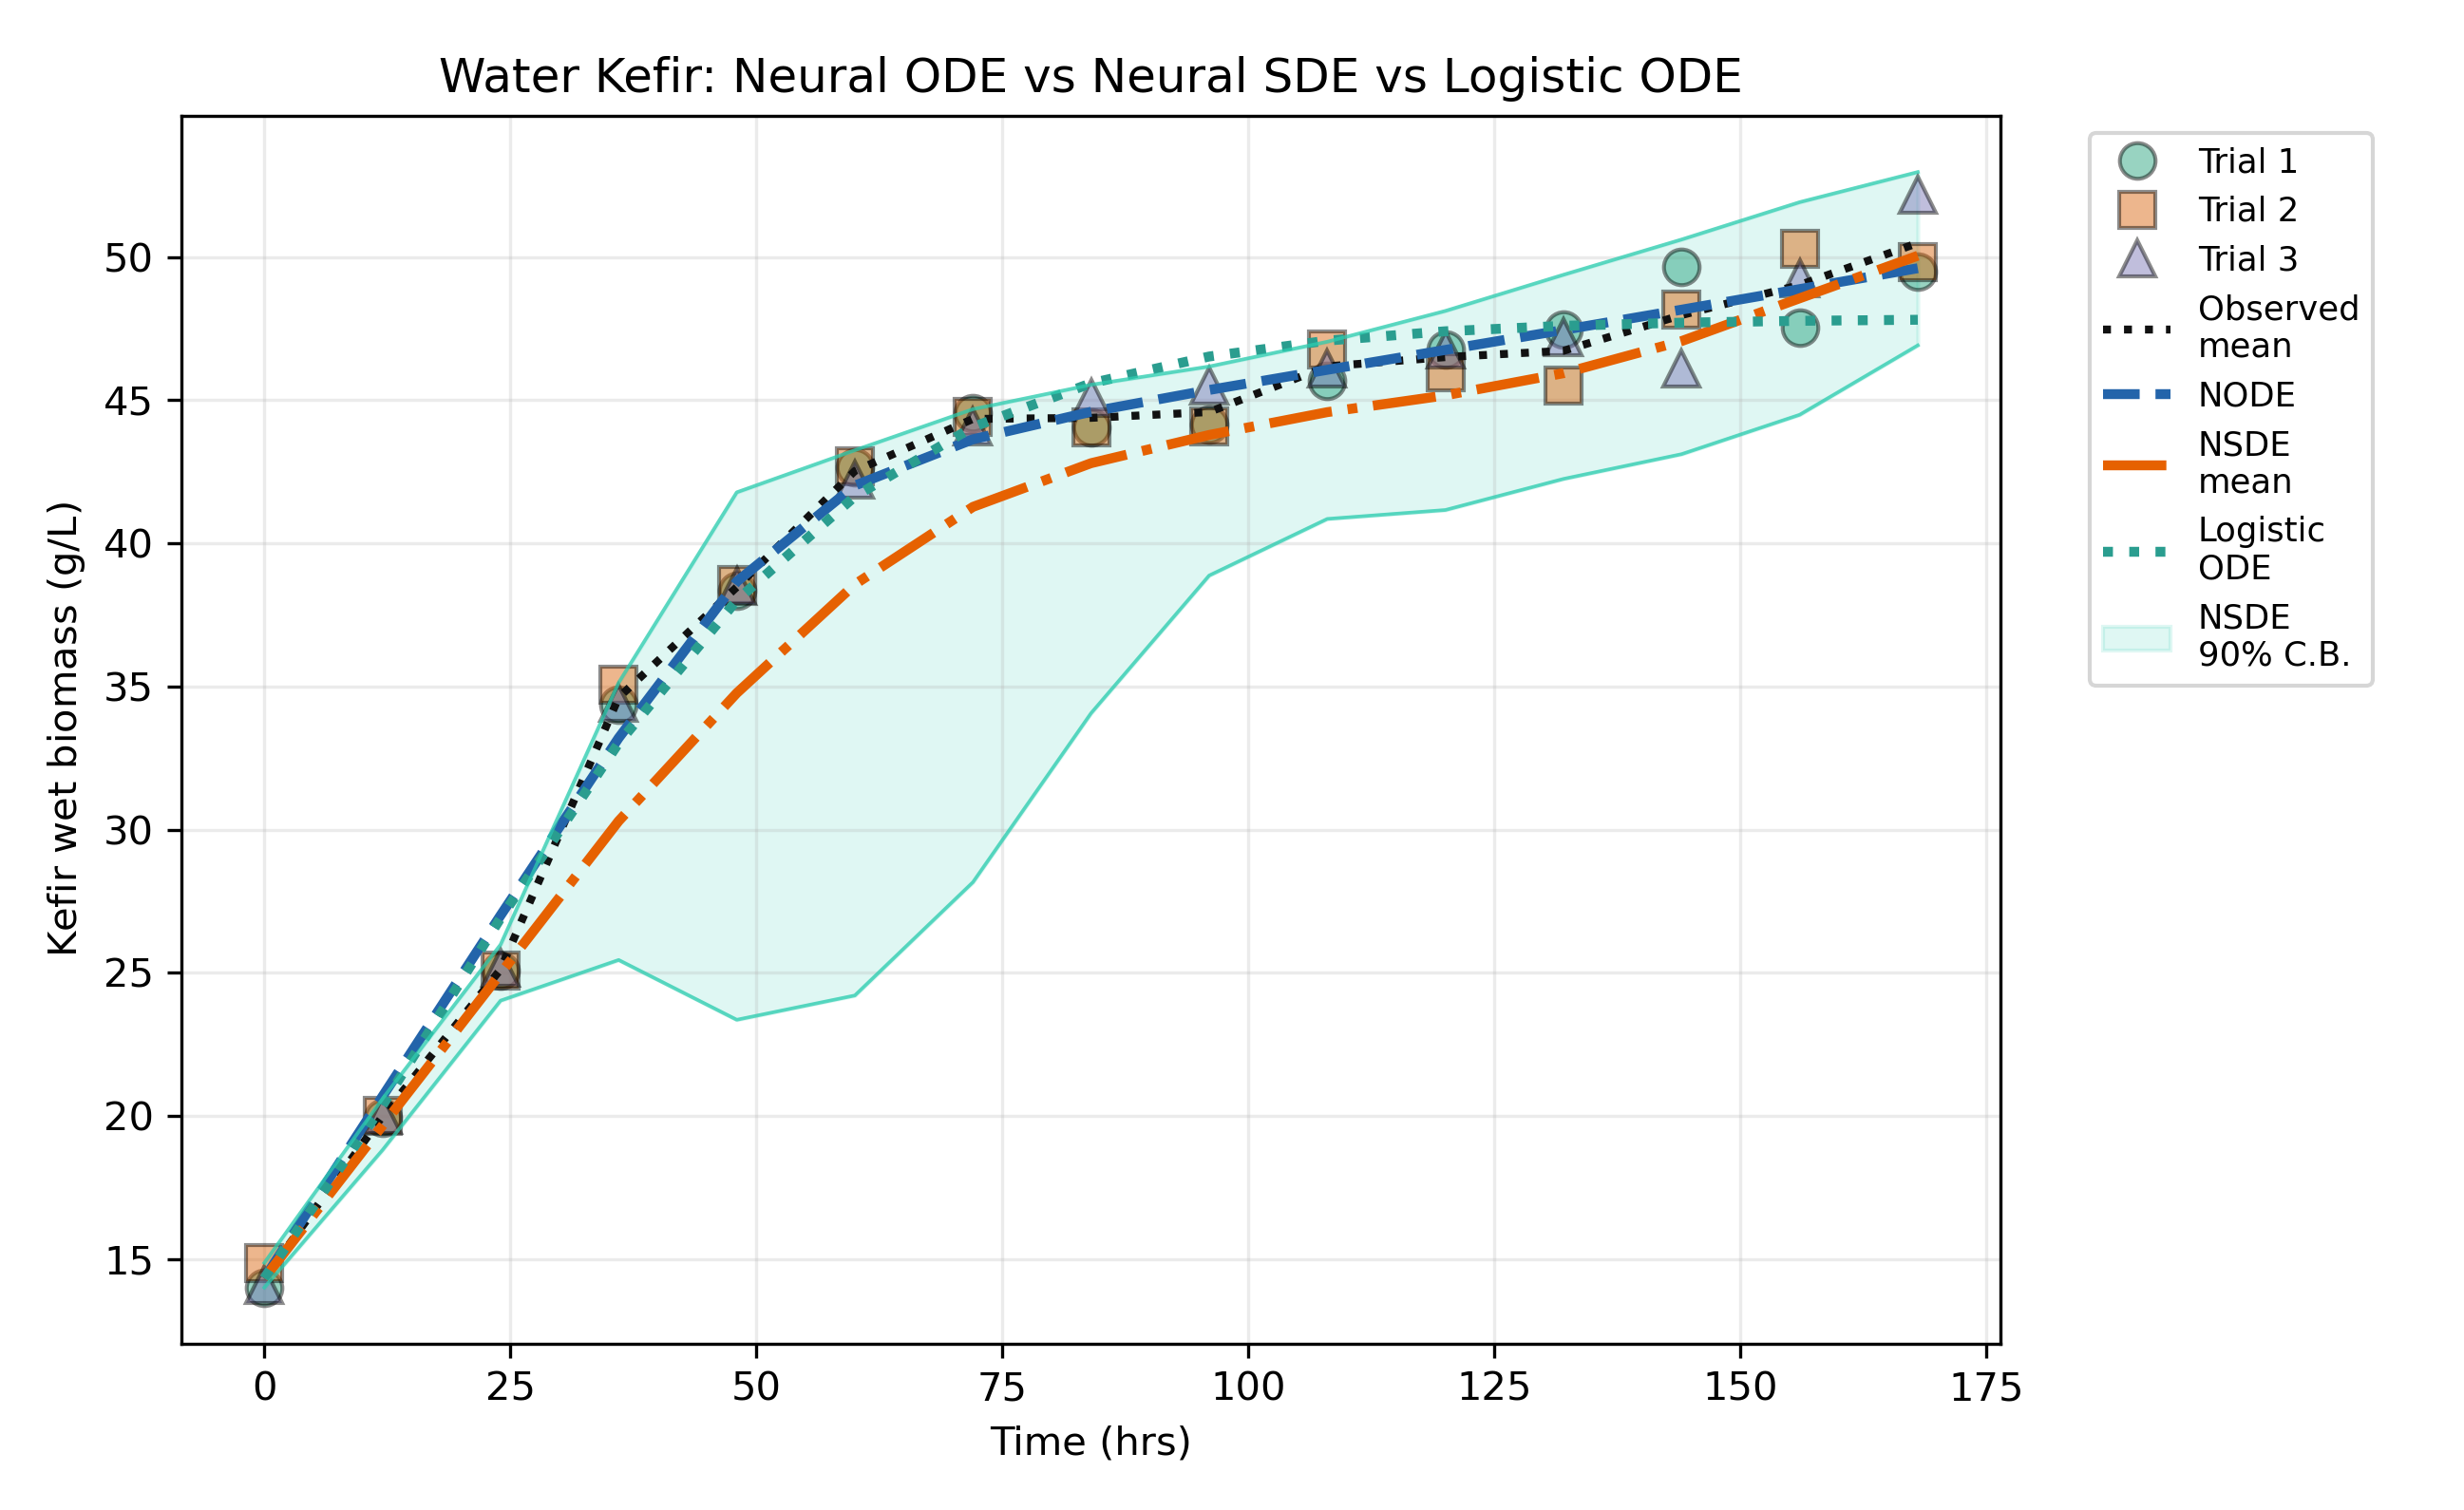
\includegraphics[width=\comparisonfigurewidth]{../results/neural_sde_comparison_outputs/water_kefir_neural_dynamics_comparison.png}
\caption{Observed trial data, the single Neural ODE population curve, fitted
mean trajectories from the comparison models, and the Neural SDE central
90 percent predictive interval. The Neural ODE is fitted as one curve against
all three trial realizations, while the logistic ODE captures the saturating
growth pattern with a much smaller parameter count. The figure uses the shared
fixed-canvas comparison layout.}
\label{fig:fit-comparison}
\end{figure}

\begin{figure}[htbp]
\centering
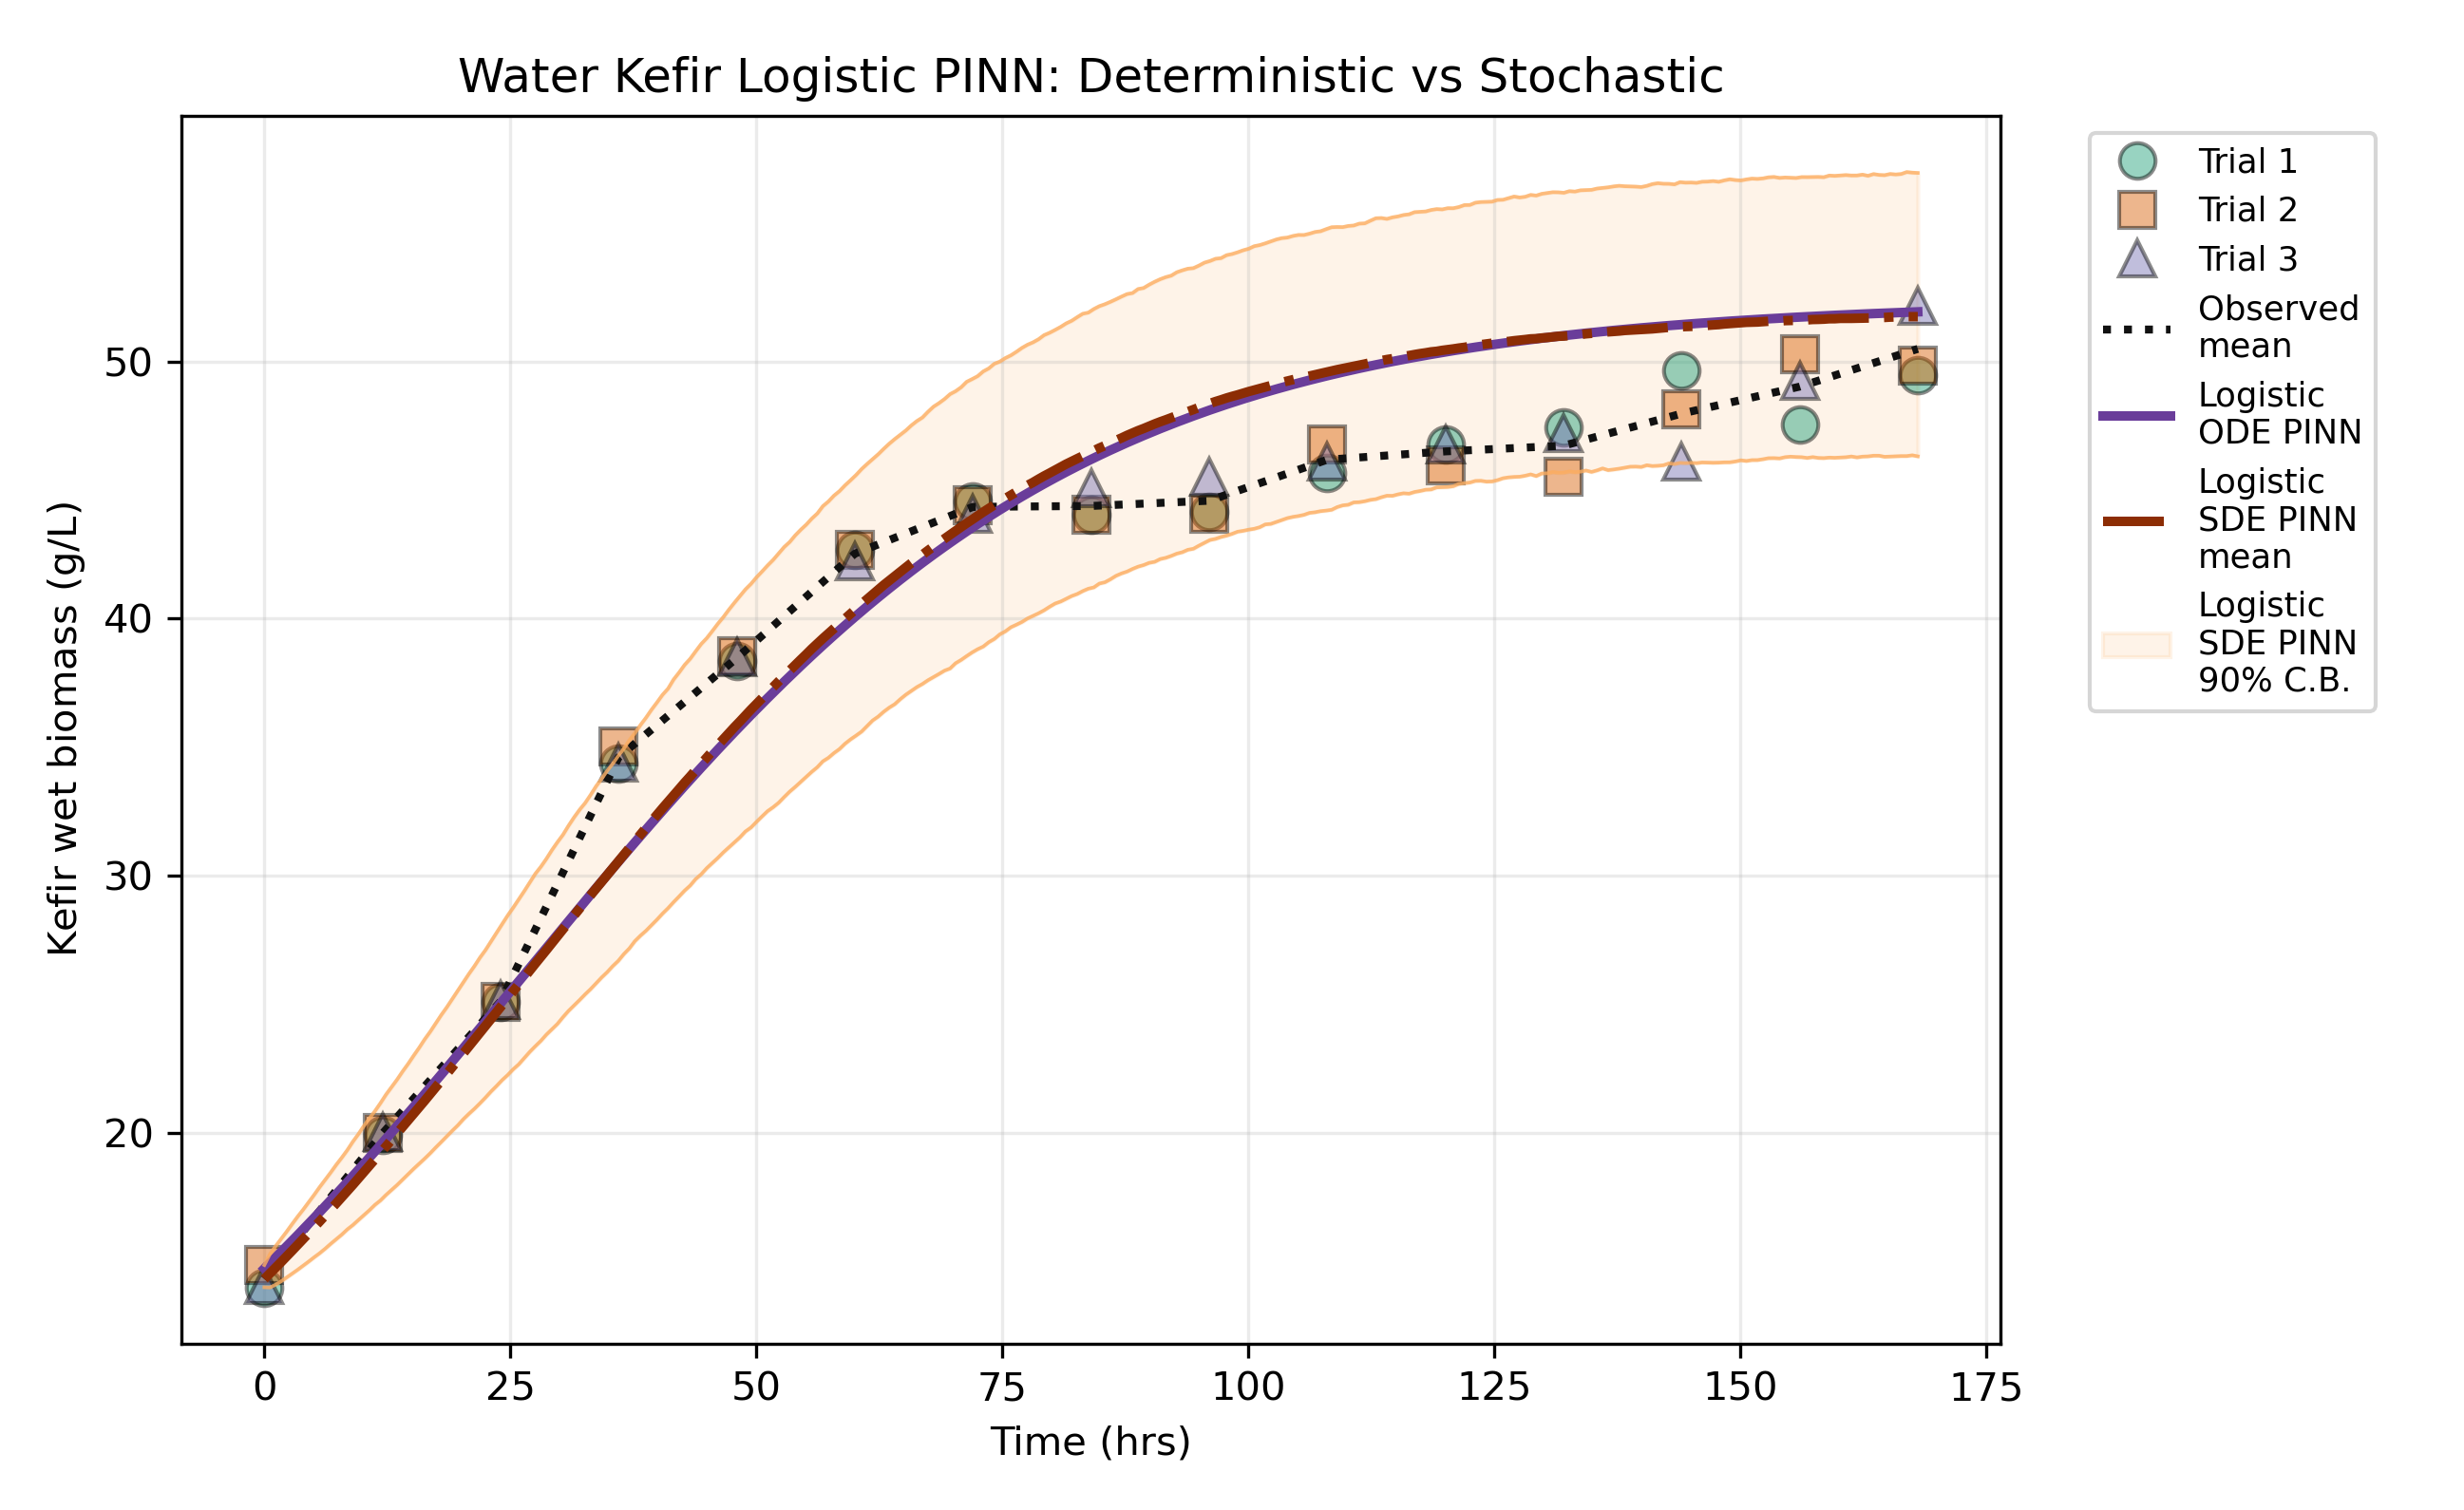
\includegraphics[width=\comparisonfigurewidth]{../results/logistic_pinn_outputs/water_kefir_logistic_pinn_comparison.png}
\caption{Observed trial data, deterministic logistic PINN population
trajectory, stochastic logistic SDE predictive mean, and central 90 percent
predictive interval. The deterministic and stochastic PINNs use the same
three-hidden-layer trajectory architecture and differ by the stochastic
transition-likelihood term used to identify $\sigma$. The line colors and
styles match the all-model comparison.}
\label{fig:logistic-pinn-comparison}
\end{figure}

\begin{figure}[htbp]
\centering
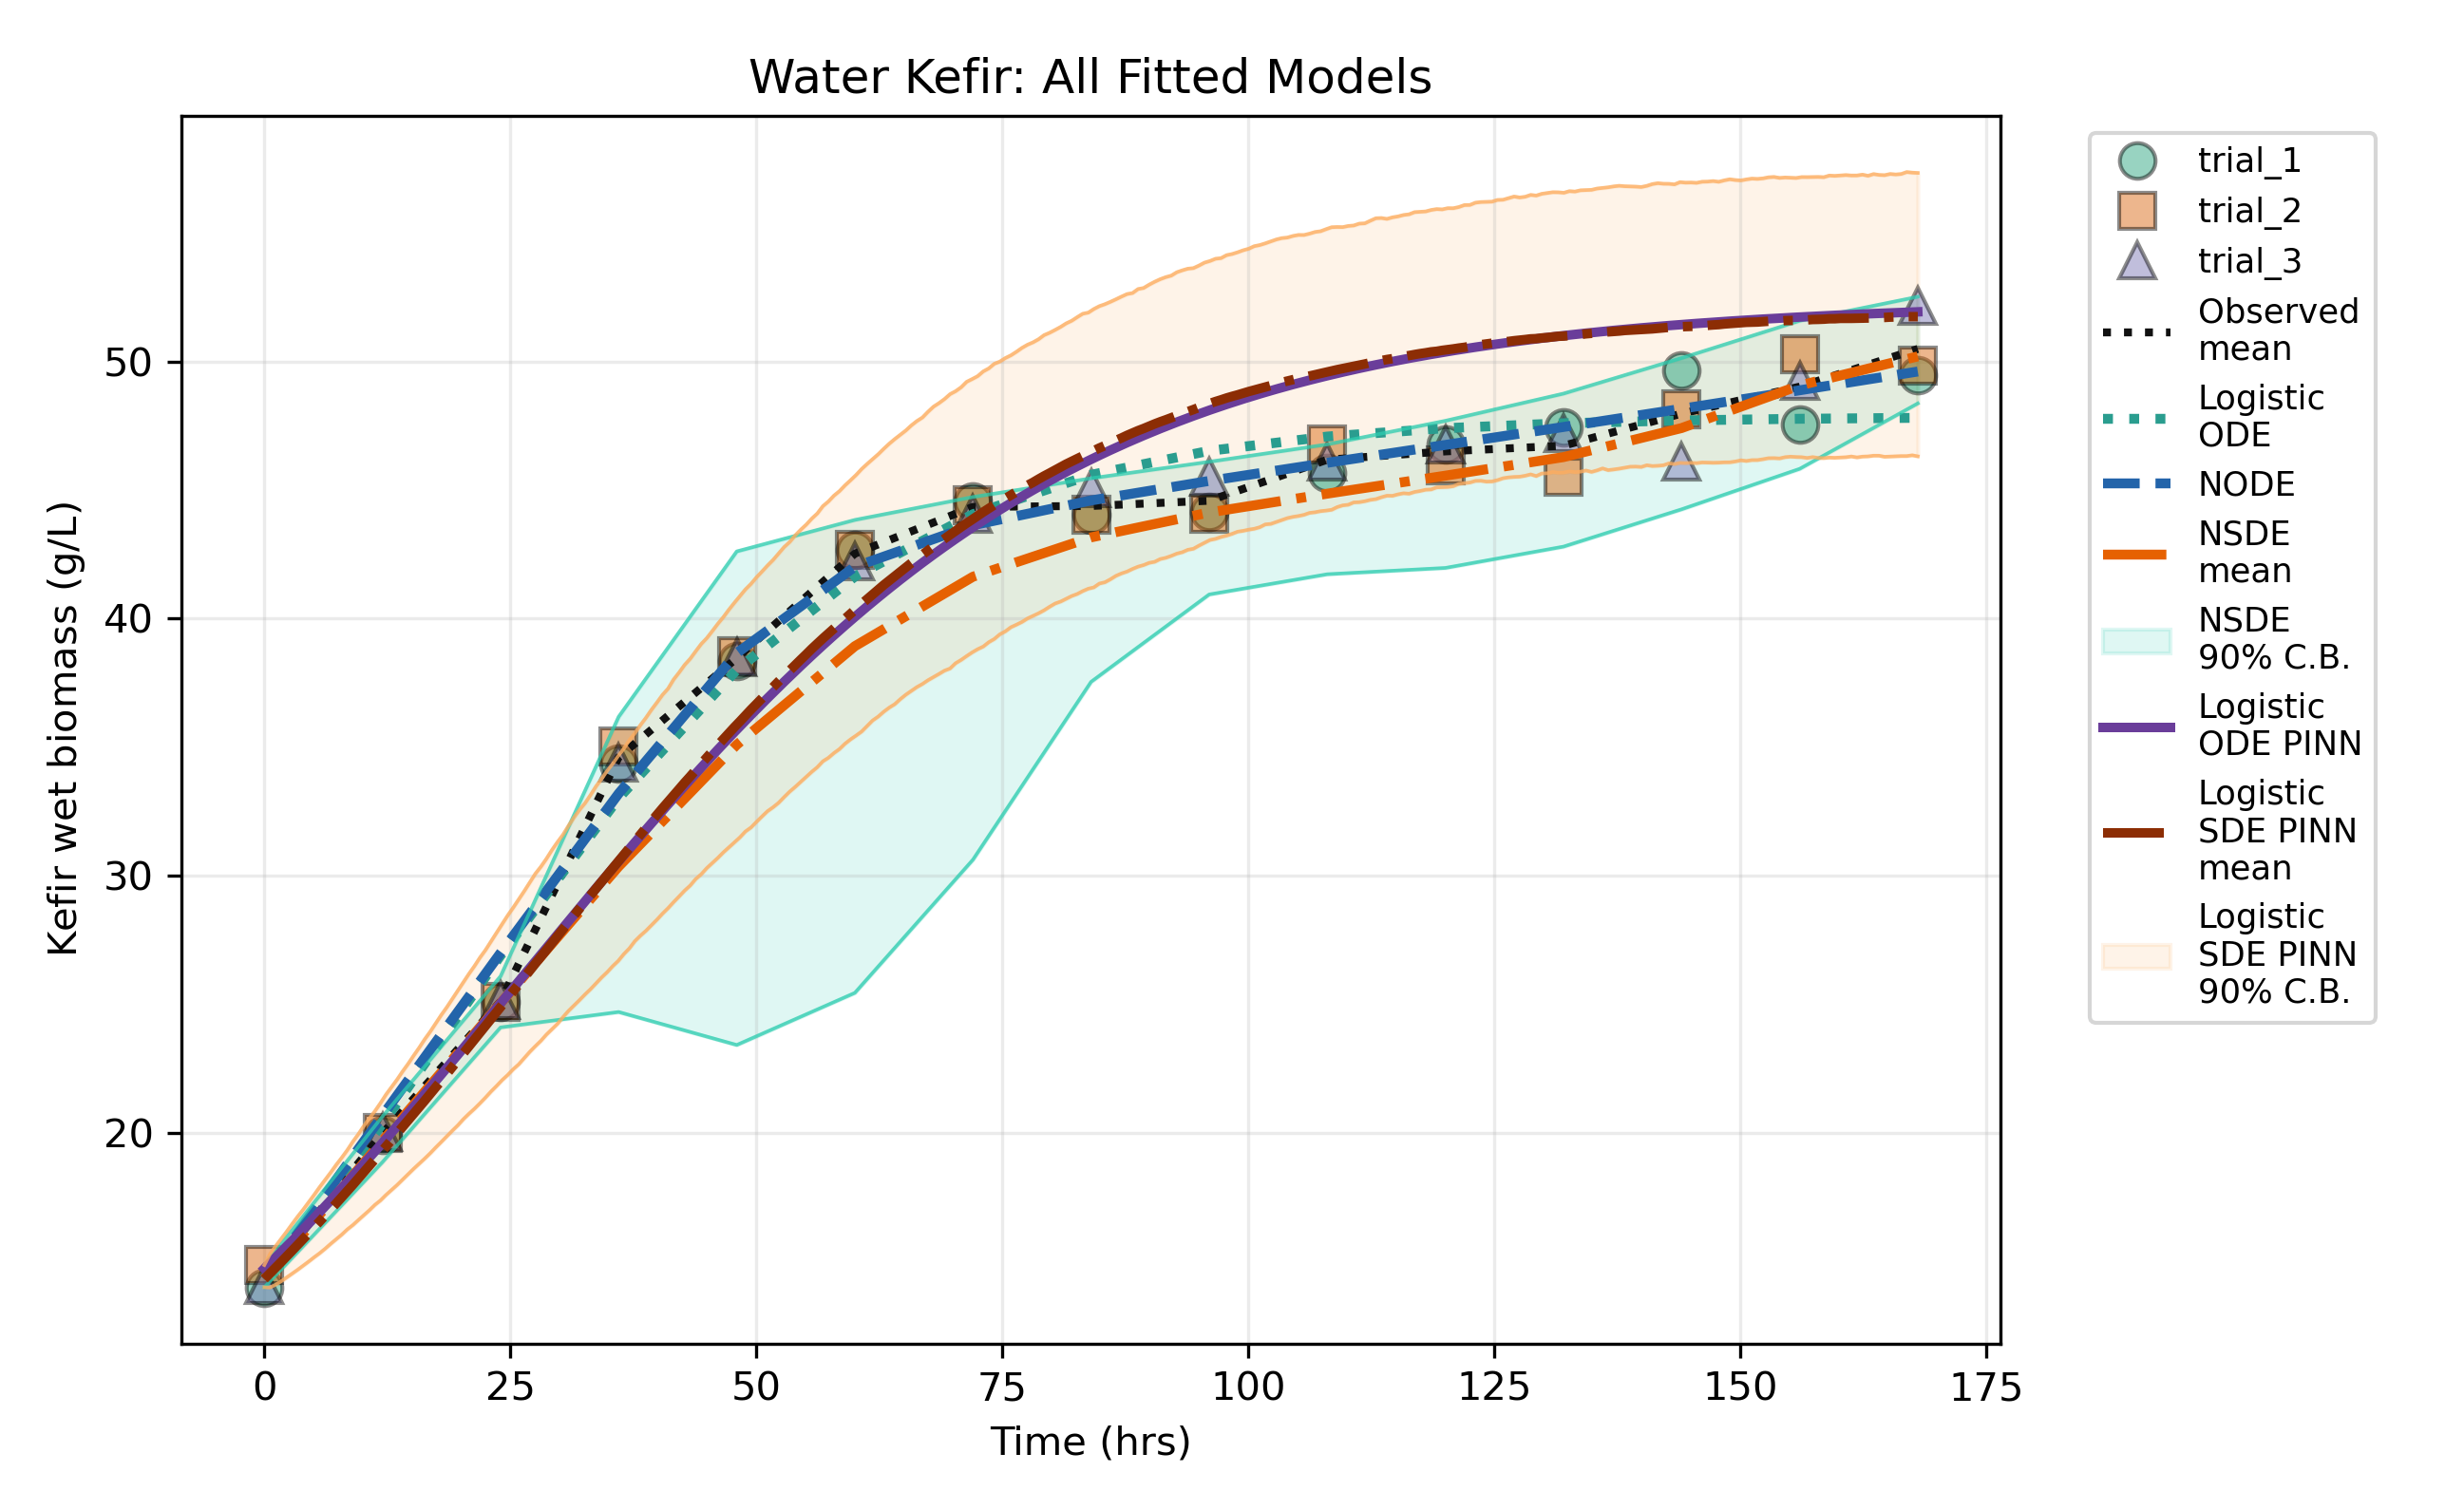
\includegraphics[width=\comparisonfigurewidth]{../results/all_model_comparison_outputs/water_kefir_all_models_comparison.png}
\caption{Combined comparison of the classical logistic ODE, Neural ODE, Neural
SDE, deterministic logistic PINN, and stochastic logistic PINN/SDE outputs. The
plot overlays the two previously separate comparison sequences on a common
original response scale so that fitted mean trajectories and predictive bands
can be visually compared without a layout change between sequence frames.}
\label{fig:all-model-comparison}
\end{figure}

\begin{figure}[htbp]
\centering
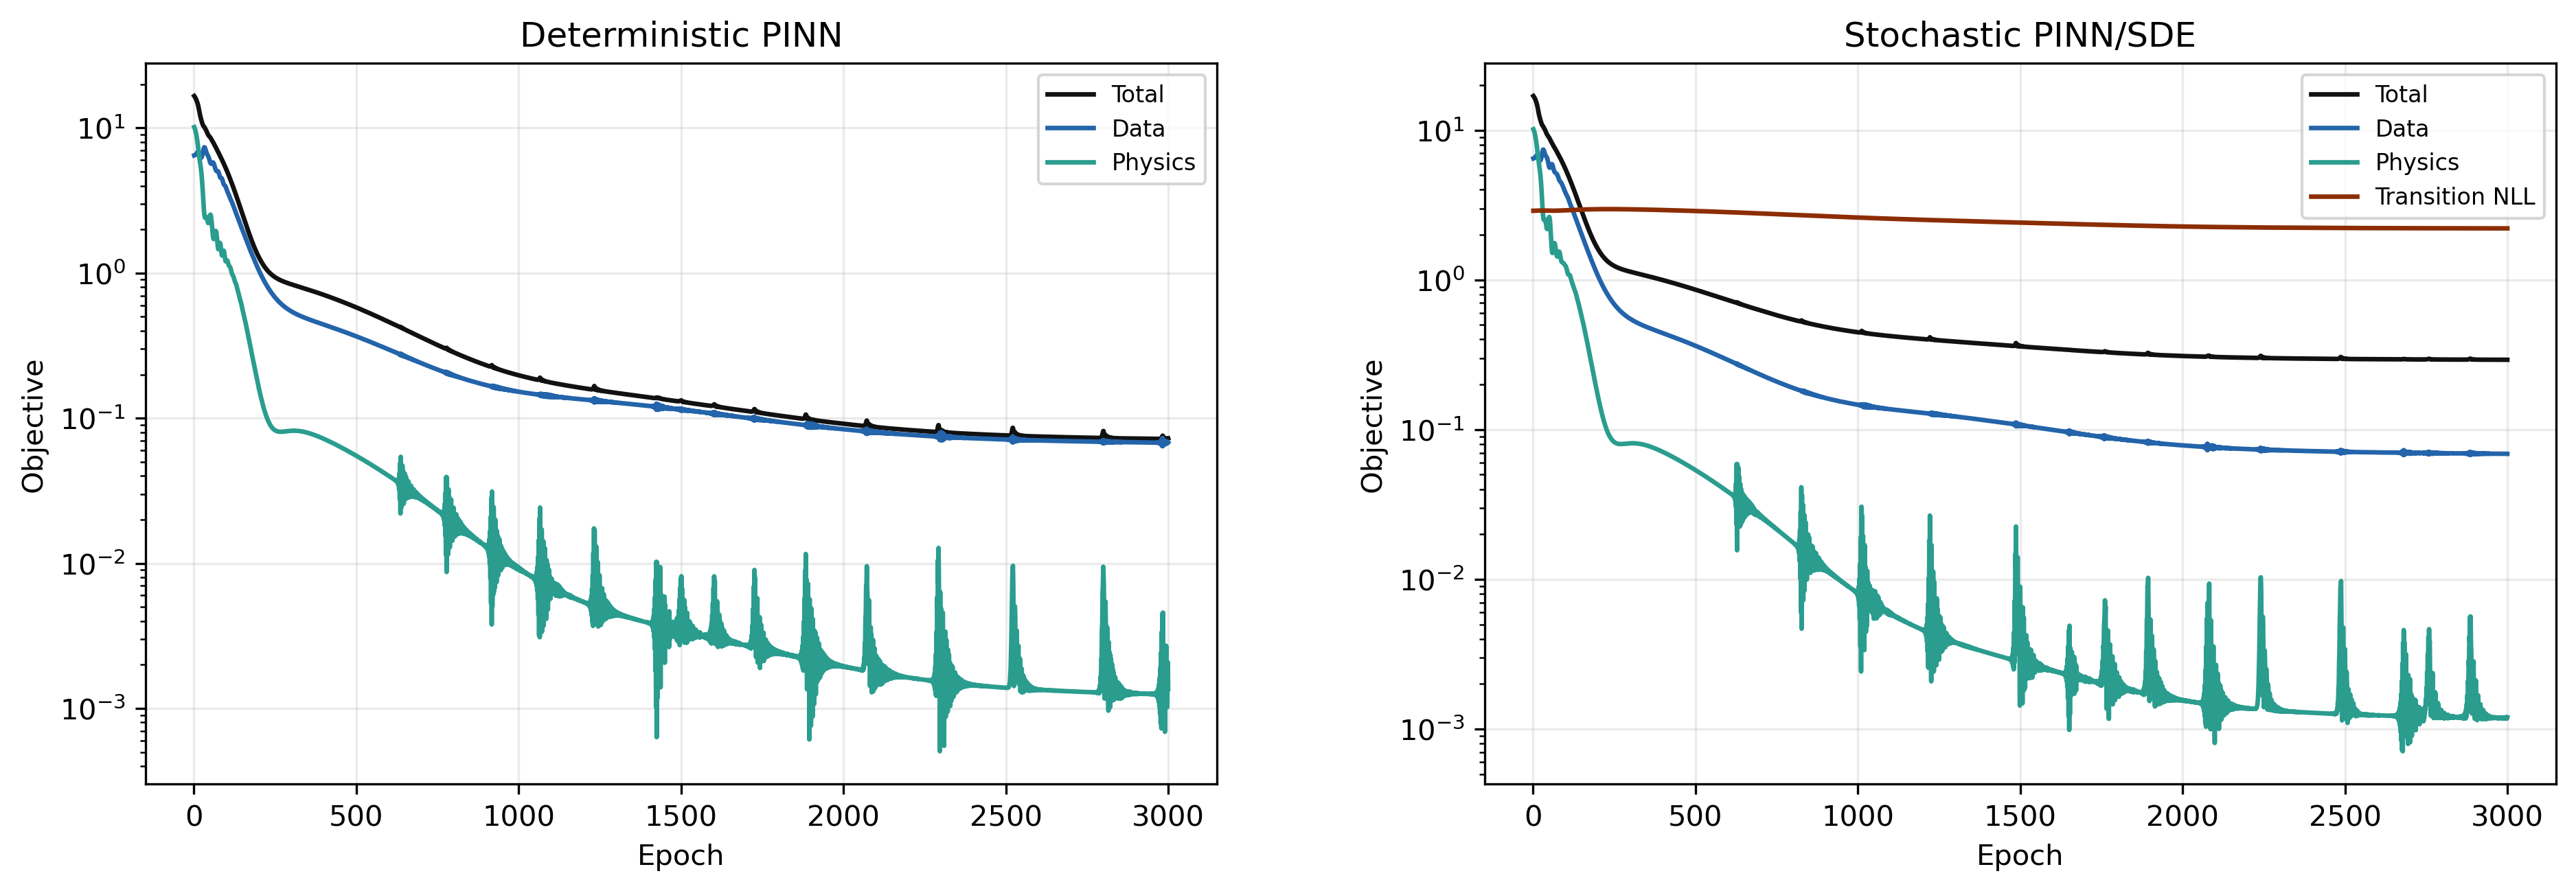
\includegraphics[width=\diagnosticfigurewidth]{../results/logistic_pinn_outputs/water_kefir_logistic_pinn_losses.png}
\caption{Training objectives for the deterministic and stochastic logistic
PINNs. The deterministic objective combines normalized data, initial-condition,
and physics residual terms. The stochastic objective adds the weighted
Euler-Maruyama transition negative log-likelihood.}
\label{fig:logistic-pinn-losses}
\end{figure}

\begin{figure}[htbp]
\centering
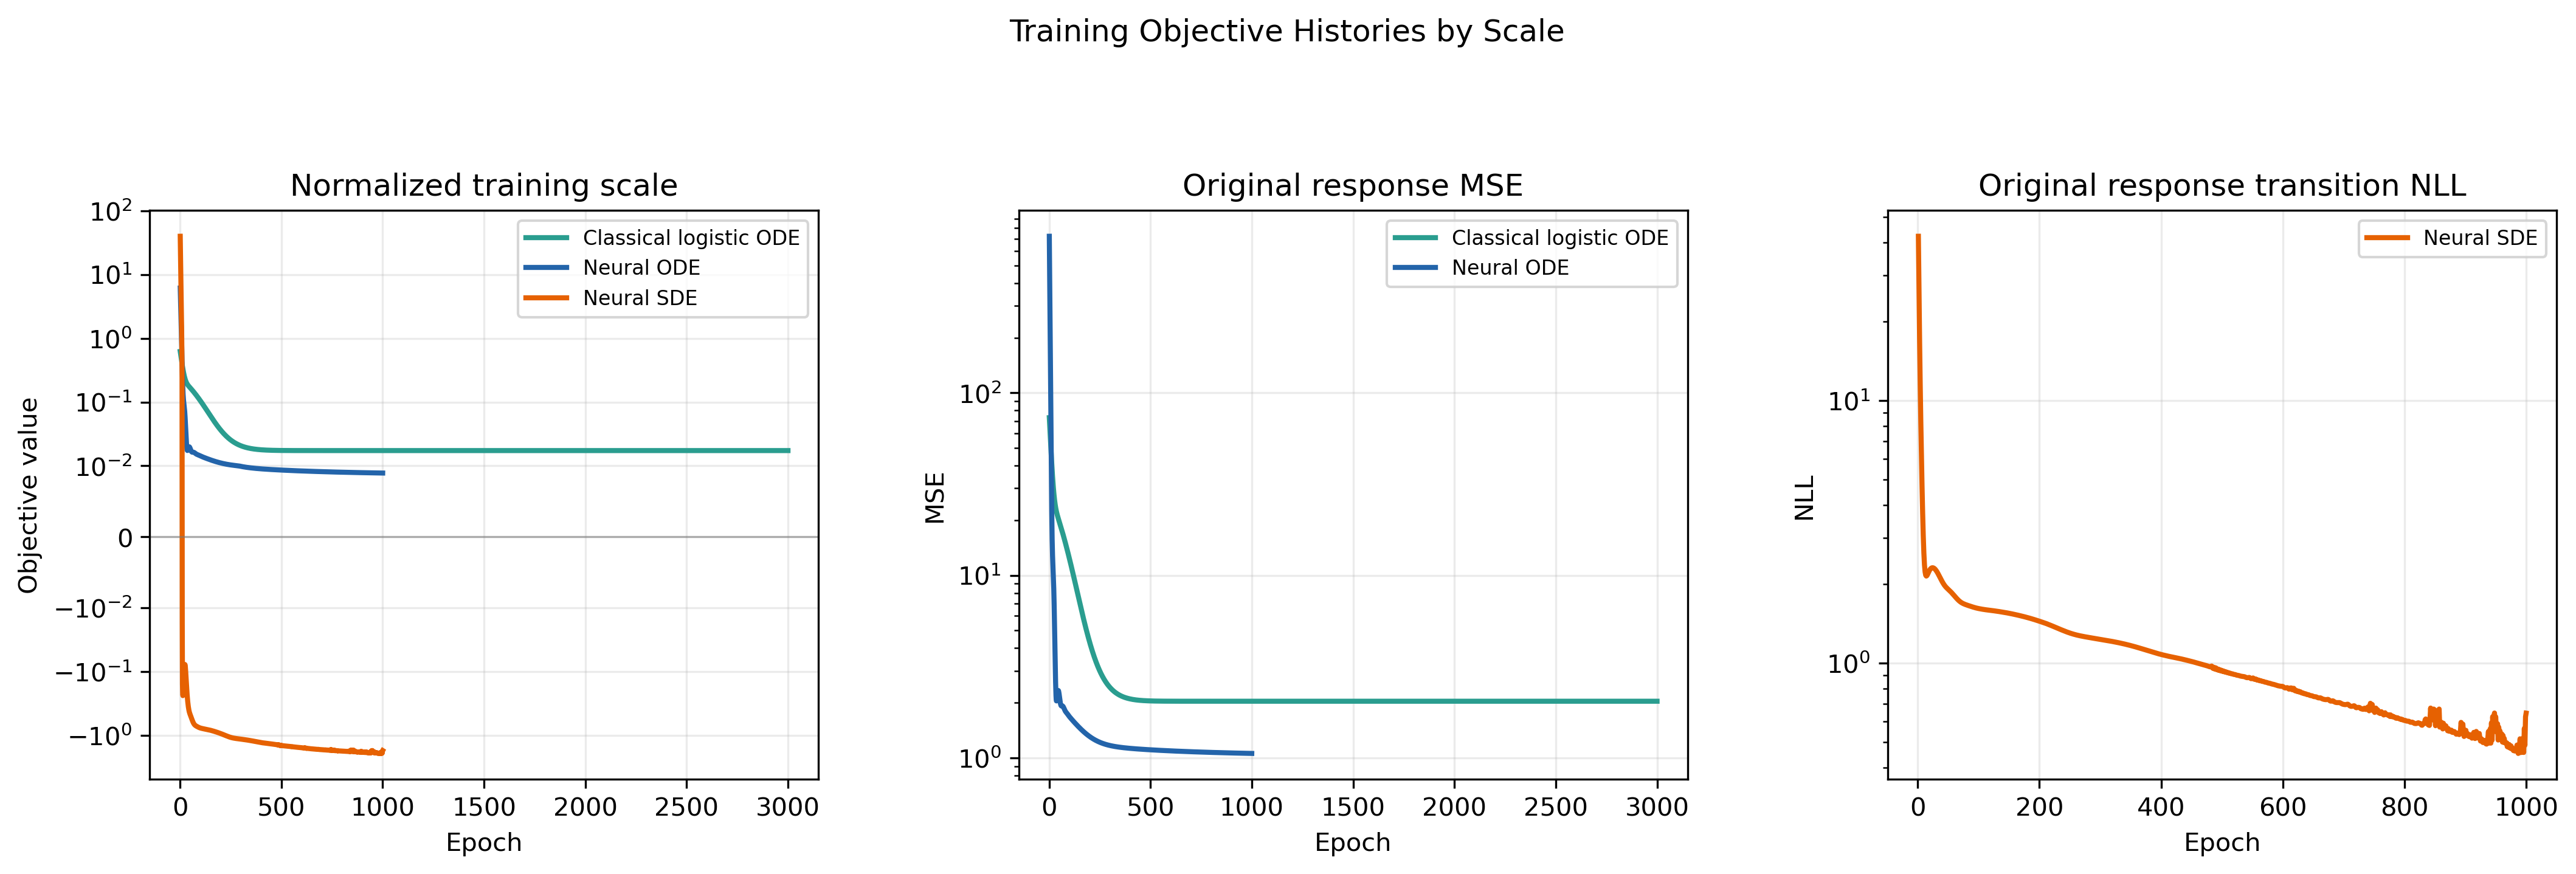
\includegraphics[width=\diagnosticfigurewidth]{../results/neural_sde_comparison_outputs/training_objectives.png}
\caption{Training objective histories from the saved experiment outputs,
re-expressed by scale. The first panel shows the objectives on normalized
training scales, the second panel compares the classical and Neural ODE MSE
histories on the original response scale, and the third panel shows the Neural
SDE transition negative log-likelihood on the original response scale. These
histories are optimization diagnostics, not direct model-comparison metrics,
because MSE and transition likelihood remain different objective types.}
\label{fig:training-objectives}
\end{figure}

\section{Reproducibility}

The original classical, Neural ODE, and Neural SDE comparison was generated by
the SDE comparison command-line tool implemented in
\path{src/kefir_models/sde_compare.py}. The deterministic and stochastic
logistic PINN comparison was generated by the logistic PINN command-line tool
implemented in \path{src/kefir_models/logistic_pinn_compare.py}. The data file
used in this directory is named \path{data/raw/waterKefirTrialsReferece.csv}.
The following command reproduces the original Neural ODE/SDE comparison from
the project root:
\begin{verbatim}
kefir-sde-compare \
  --data-path data/raw/waterKefirTrialsReferece.csv \
  --output-dir outputs/neural_sde_comparison_outputs \
  --classical-epochs 3000 \
  --classical-learning-rate 5e-2 \
  --ode-epochs 1000 \
  --ode-learning-rate 1e-2 \
  --sde-epochs 1000 \
  --sde-learning-rate 5e-3 \
  --hidden-units 32 \
  --hidden-layers 2 \
  --weight-decay 1e-4 \
  --min-diffusion 1e-3 \
  --ode-method rk4 \
  --sde-paths 1000 \
  --interval-level 0.90 \
  --seed 7 \
  --device auto \
  --plot
\end{verbatim}

The following command reproduces the logistic PINN inverse-problem outputs:
\begin{verbatim}
kefir-logistic-pinn-compare \
  --config configs/logistic_pinn_config_reference.json
\end{verbatim}

The following plotting-only command builds the third step-by-step sequence that
overlays the classical logistic ODE, Neural ODE, Neural SDE, deterministic
logistic PINN, and stochastic logistic PINN/SDE outputs:
\begin{verbatim}
kefir-plot-all-models \
  --neural-comparison-csv \
    outputs/neural_sde_comparison_outputs/water_kefir_neural_dynamics_comparison.csv \
  --pinn-comparison-csv \
    logistic_pinn_outputs/water_kefir_logistic_pinn_comparison.csv \
  --pinn-dense-csv \
    logistic_pinn_outputs/water_kefir_logistic_pinn_dense.csv \
  --output-dir outputs/all_model_comparison_outputs \
  --interval-level 0.90
\end{verbatim}

The updated PNGs in this report use the shared style and fixed-canvas save
helpers in \path{src/kefir_models/plot_style.py}. The comparison figures are
written with the same $2594\times1590$ pixel canvas, while the wider loss and
objective-history diagnostics are saved with tight bounds.

Equivalently, the expanded logistic PINN configuration is:
\begin{verbatim}
kefir-logistic-pinn-compare \
  --data-path data/raw/waterKefirTrialsReferece.csv \
  --output-dir logistic_pinn_outputs \
  --deterministic-epochs 3000 \
  --stochastic-epochs 3000 \
  --learning-rate 5e-3 \
  --hidden-units 32 \
  --hidden-layers 3 \
  --collocation-points 128 \
  --physics-weight 1.0 \
  --initial-weight 1.0 \
  --transition-weight 0.1 \
  --initial-diffusion 0.02 \
  --sde-paths 5000 \
  --interval-level 0.90 \
  --plot-points 300 \
  --seed 7 \
  --device auto \
  --plot
\end{verbatim}

The main output files used in this report are:
\begin{itemize}
  \item \path{outputs/neural_sde_comparison_outputs/model_comparison_metrics.csv},
  \item \path{outputs/neural_sde_comparison_outputs/classical_logistic_parameters.csv},
  \item \path{outputs/neural_sde_comparison_outputs/water_kefir_neural_dynamics_comparison.csv},
  \item \path{outputs/neural_sde_comparison_outputs/water_kefir_neural_dynamics_comparison.png},
  \item \path{outputs/neural_sde_comparison_outputs/training_objective_scales.csv},
  \item \path{outputs/neural_sde_comparison_outputs/training_objectives.png},
  \item \path{outputs/all_model_comparison_outputs/water_kefir_all_models_comparison.png},
  \item \path{logistic_pinn_outputs/water_kefir_logistic_pinn_metrics.csv},
  \item \path{logistic_pinn_outputs/water_kefir_logistic_pinn_parameters.csv},
  \item \path{logistic_pinn_outputs/water_kefir_logistic_pinn_comparison.csv},
  \item \path{logistic_pinn_outputs/water_kefir_logistic_pinn_comparison.png},
  \item \path{logistic_pinn_outputs/water_kefir_logistic_pinn_losses.png}.
\end{itemize}

\bibliographystyle{plainnat}
\bibliography{kefir_model_comparison_references}

\end{document}
